\chapter{Modelagem UML}

\section{Requisitos funcionais}

\begin{enumerate}[topsep=0pt, partopsep=0pt, itemsep=0pt]
  \item A estação base deve ler a posição do robô e atualizar a interface gráfica automaticamente. Representado pelo requisito funcional: \textbf{"Estação base mostra na interface gráfica a posição do robô - RF01"}
  \item A estação base deve ler as posições dos novos obstáculos detectados e atualizar a interface gráfica automaticamente. Representado pelo requisito funcional: \textbf{"Estação base mostra na interface gráfica os novos obstáculos detectados pelo robô - RF02"}
  \item A estação base deve mostrar na interface gráfica a imagem captada pela webcam. Representado pelo requisito funcional: \textbf{"Estação base atualiza a imagem captada pela webcam - RF03"}
  \item O usuário pode controlar os seguintes quatro movimentos do robô: movimentar para frente, para trás, para a esquerda ou para a direita. Representado pelo requisito funcional: \textbf{"O usuário pode movimentar o robô - RF04"}
  \item A estação base deve ser capaz de estabelecer conexão com o robô, informando o usuário caso a conexão ocorra com sucesso ou não. Representado pelo requisito funcional \textbf{"O usuário pode estabelecer a conexão entre o robô e a estação base - RF05"}
\end{enumerate}

\section{Requisitos não funcionais}

\begin{enumerate}[topsep=0pt, partopsep=0pt, itemsep=0pt]
  \item O usuário poderá salvar o caminho percorrido pelo robô. Representado pelo requisito não funcional: \textbf{"O usuário pode salvar o caminho percorrido - RNF01"}
  \item O usuário poderá carregar o caminho percorrido pelo robô. Representado pelo requisito não funcional: \textbf{"O usuário pode carregar o caminho percorrido - RNF02"}
  \item A imagem transmitida pela câmera do robô deve ser colorida. Representado pelo requisito não funcional: \textbf{"O robô deve enviar os dados de vídeo coloridos para a estação base - RNF03"}
  \item O robô deve transmitir as imagens de sua câmera em tempo real. Representado pelo requisito não funcional: \textbf{"O robô pode transmitir os dados de vídeo captados pela câmera em tempo real - RNF04"}
  \item O método de entrada do usuário deve se dar por meio de interface gráfica com o auxílio do mouse. Representado pelo requisito não funcional: \textbf{"O usuário pode interagir com o robô por meio do mouse - RNF05"}
  \item O método de entrada do usuário deve se dar por meio de interface gráfica com o auxílio do teclado. Representado pelo requisito não funcional: \textbf{"O usuário pode interagir com o robô por meio do teclado - RNF06"}
\end{enumerate}


\subsection{Casos de uso}

\begin{enumerate}[topsep=0pt, partopsep=0pt, itemsep=0pt]
  \item Movimentação do robô pelo usuário. Representado pelo caso de uso: \textbf{"Movimentar robô - UC01"}
  \item Parada do robô solicitada pelo usuário. Representado pelo caso de uso: \textbf{"Parar o robô - UC02"}
  \item Solicitação de estabelecimento de conexão com o robô. \textbf{"Estabelecer conexão com o robô - UC03"}
  \item Alteração na velocidade do robô solicitada pelo usuário. \textbf{"Alterar velocidade do robô - UC04"}
  \item Alteração da posição do robô na interface gráfica segundo os dados lidos do robô. Representado pelo caso de uso: \textbf{"Mostrar posição do robô na interface gráfica - UC05"}
  \item Inclusão de novos obstáculos e suas posições lidos do robô. Representado pelo caso de uso: \textbf{"Mostrar posição dos novos obstáculos detectados na tela - UC06"}
  \item Consulta da documentação do robô solicitada pelo usuário. Representado pelo caso de uso: \textbf{"Consultar documentação do robô - UC07"}
\end{enumerate}

\begin{figure}[H]
  \centering
  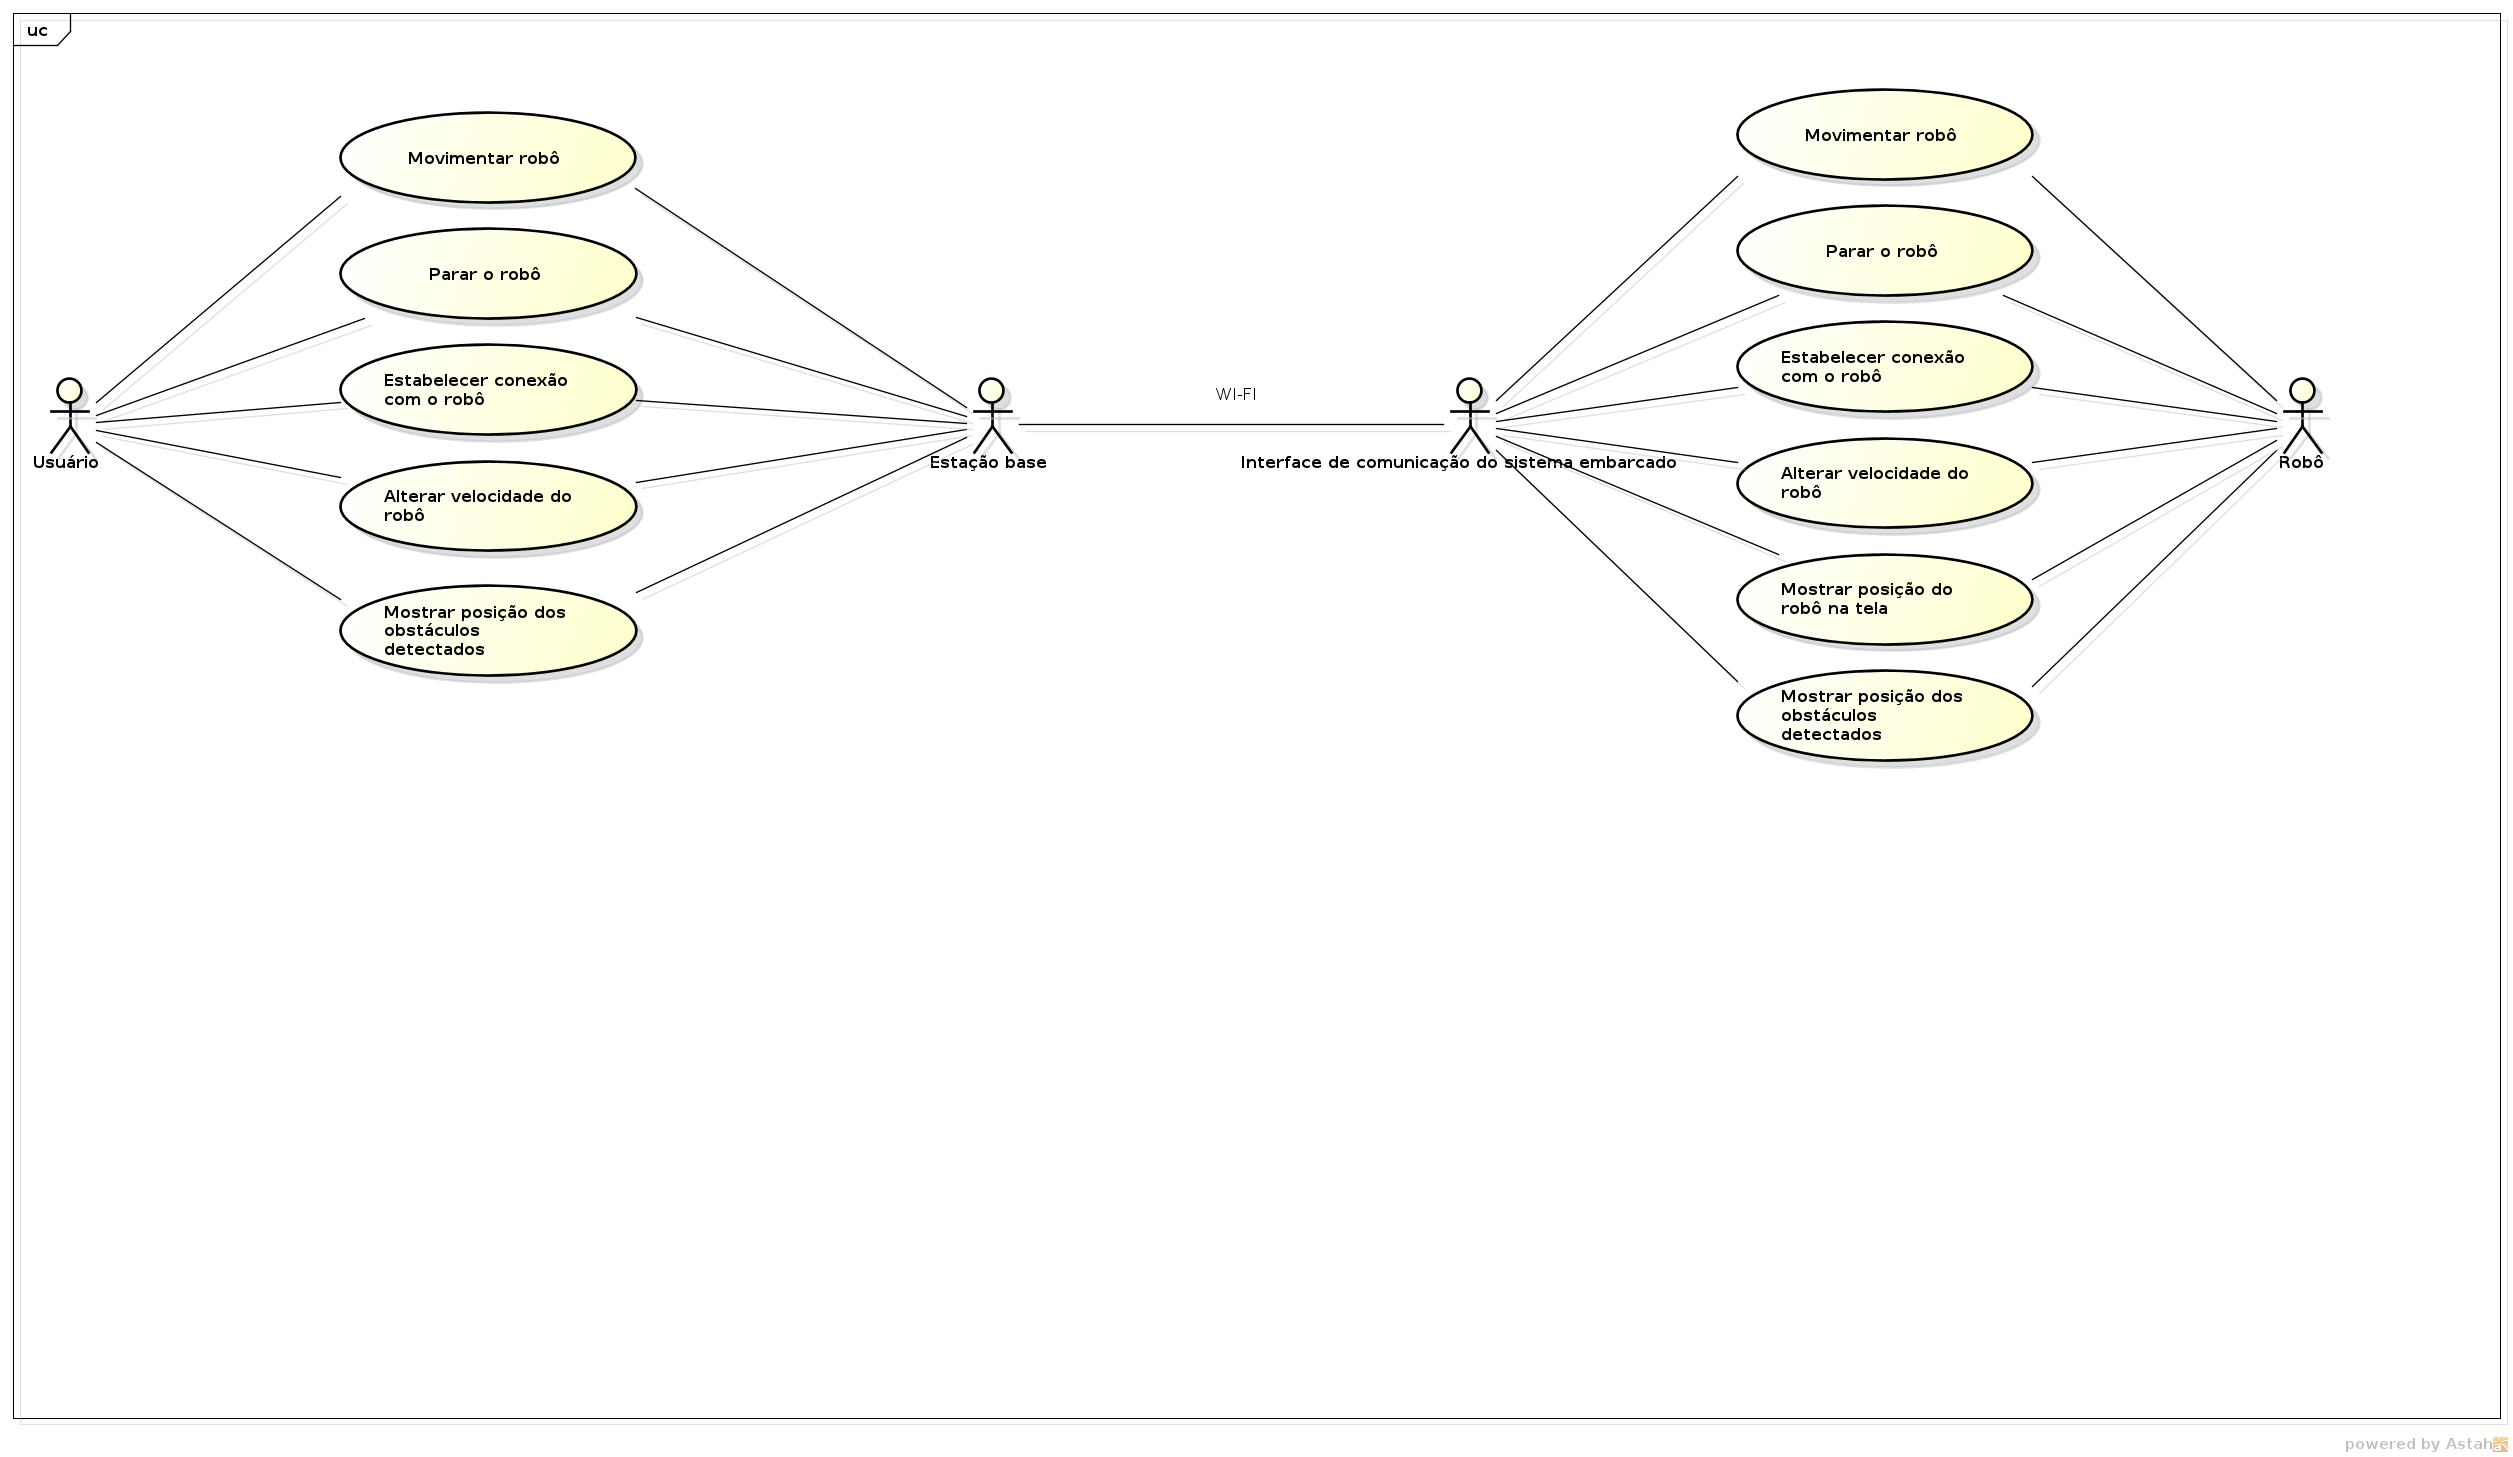
\includegraphics[width=\textwidth, keepaspectratio]{./figuras/diagrama_casos_de_uso_v2.png}
  \caption{Diagrama de casos de uso}
  \label{fig:diagrama_casos_de_uso}
\end{figure}

\section{Descrição das classes}

\subsection{Pacote visual}

O software da estação base do robô foi dividido em cinco pacotes:  visual, controle, comunicação, controle.robo e interface gráfica. Estes serão descritos com suas respectivas classes na Tabela \ref{tab:pacote_visual}.

\begin{table}[h]
  \centering
  \caption{Pacote visual}
    \begin{tabular}{p{6cm}p{8cm}}
    \toprule
    \textbf{Classe} & \textbf{Descrição} \\ \hline
    \midrule
    Viewer2D & Responsável por exibir os objetos Drawable2D. Possui recursos de pan, zoom e rotate.   \\ \hline
    Drawable2D & Interface genérica para objetos visuais que podem ser desenhados em um Viewer2D. \\ \hline
    EscalaDrawable & Responsável por desenhar uma escala gráfica. \\ \hline
    RoboDrawable & Responsável por desenhar o robô na interface gráfica. \\ \hline
    RoboTrilhaDrawable & Responsável por desenhar a trilha percorrida pelo robô na interface gráfica. \\ \hline
    ObstaculosDrawable & Responsável por desenhar os pontos de cada obstáculo na interface gráfica. \\ \hline
    EscalaDrawableProp & Contém as propriedades visuais de desenho da escala. \\ \hline
    RoboDrawableProp & Contém as propriedades visuais de desenho do robô \\ \hline
    RoboTrilhaDrawableProp & Contém as propriedades visuais de desenho da trilha do robô. \\ \hline
    ObstaculosDrawableProp & Contém as propriedades visuais de desenho dos obstáculos. \\ \hline
    Ponto & Representa um ponto de cordenadas cartesianas. \\ \hline
    \bottomrule
    \end{tabular}%
  \label{tab:pacote_visual}%
\end{table}%

\subsection{Pacote controle}

Este pacote consiste de toda a parte da estação base que controla as informações essenciais do robô. Conta com as seguintes classes: Mapa, Obstaculos, Robo, ControleSensores, Posinfo, SensorIR e ControleCamera. Na Tabela \ref{tab:pacote_controle} estão descritas as classes deste pacote.

\begin{table}[h]
  \centering
  \caption{Pacote de controle}
    \begin{tabular}{p{6cm}p{8cm}}
    \toprule
    \textbf{Classe} & \textbf{Descrição} \\ \hline
    \midrule
    Mapa  & Responsável por representar o mapa. Armazena as informações essenciais do robô e dos obstáculos detectados. \\ \hline
    Obstaculos & Responsável por conter os obstáculos detectados pelo robô. \\ \hline
    Robo  & Responsável por representar o robô, este contêm largura, comprimento e centro de movimento (ponto central entre as duas rodas). \\ \hline
    ControleSensores & Responsável em atualizar a posição do robô e dos pontos que representão os obstáculos, de acordo com as leituras feitas pelos sensores. \\ \hline
    Posinfo & Responsável por conter as informações de uma posição do robô. \\ \hline
    SensorIR & Responsável por representar um sensor IR do robô. \\ \hline
    ControleCamera & Responsável por controlar as imagens da câmera e o status do recebimento das imagens. \\ \hline
    \bottomrule
    \end{tabular}%
  \label{tab:pacote_controle}%
\end{table}%

\subsection{Pacote comunicação}

Este pacote consiste em toda a parte de comunicação da estação base com o robô e conta com as seguintes classes: ClientCommandInterpreter, ClientConnection, ClientReceiver, ClientSender, ServerCommandInterpreter, ServerListener, ServerSender, ServerReceiver e Message. Na Tabela \ref{tab:pacote_comunicacao} estão descritas as classe deste pacote.

\begin{table}[h]
  \centering
  \caption{Pacote de comunicação}
    \begin{tabular}{p{6cm}p{8cm}}
    \toprule
    \textbf{Classe} & \textbf{Descrição} \\ \hline
    \midrule
    ClientCommandInterpreter & Responsável pela interpretação dos comandos do cliente. Os comandos recebidos são inseridos em uma fila, de modo a serem posteriormente executados pela thread. \\ \hline
    ClientConnection & Responsável por efetuar a gerência da conexão do cliente (estação base) com o servidor (robô). \\ \hline
    ClientReceiver & Responsável por receber mensagens de um host de uma conexão. \\ \hline
    ClientSender & Responsável por enviar mensagens ao host de uma conexão. \\ \hline
    ServerCommandInterpreter & Responsável pela interpretação dos comandos do servidor. Os comandos recebidos são inseridos em uma fila, de modo a serem posteriormente executados pela thread. \\ \hline
    ServerListener & Responsável por escutar as novas conexões de clientes. \\ \hline
    ServerSender & Responsável por enviar mensagens ao host de uma conexão. \\ \hline
    ServerReceiver & Responsável por receber mensagens de um host de uma conexão. \\ \hline
    Message & Contém uma mensagem a ser enviada por um Sender. \\ \hline
    \bottomrule
    \end{tabular}%
  \label{tab:pacote_comunicacao}%
\end{table}%

\subsection{Pacote interface gráfica}

Este pacote consiste em toda a interface gráfica do sistema e conta com as seguintes classes: JanelaConexao, JanelaPrincipal e JanelaSensores. Na Tabela \ref{tab:pacote_interface_grafica} estão descritas as classes deste pacote.

\begin{table}[h]
  \centering
  \caption{Pacote de interface gráfica}
    \begin{tabular}{p{6cm}p{8cm}}
    \toprule
    \textbf{Classe} & \textbf{Descrição} \\ \hline
    \midrule
    JanelaConexao & Responsável por conter a janela com as informações e configurações da conexão com o Bellator. \\ \hline
    JanelaPrincipal & Responsável por desenhar a janela principal da interface gráfica do Bellator. \\ \hline
    JanelaSensores & Responsável por desenhar a janela responsável pela configuração dos sensores. \\ \hline
    \bottomrule
    \end{tabular}%
  \label{tab:pacote_interface_grafica}%
\end{table}%

\subsection{Pacote controle do robô}

Este pacote consiste de toda a parte do sistema embarcado que gerencia os sensores e atuadores do robô. Conta com as seguintes classes: SensorsManager, WebcamManager e EnginesManager. Na Tabela \ref{tab:pacote_controle_robo} serão descritas as classes deste pacote.

\begin{table}[h]
  \centering
  \caption{Pacote de controle de robô}
    \begin{tabular}{p{6cm}p{8cm}}
    \toprule
    \textbf{Classe} & \textbf{Descrição} \\ \hline
    \midrule
    SensorsManager & Responsável por gerenciar a coleta de informações dos sensores do robô. \\ \hline
    WebcamManager & Responsável por gerenciar a captura de imagens da webcam. \\ \hline
    EnginesManager & Responsável por gerenciar a ação dos motores do robô. \\ \hline
    \bottomrule
    \end{tabular}%
  \label{tab:pacote_controle_robo}%
\end{table}%



\section{Diagrama de classes}

A Figura \label{fig:diagrama_classes} mostra o diagrama de classes tanto da estação base, quanto do software embarcado.

\begin{figure}[H]
  \centering
  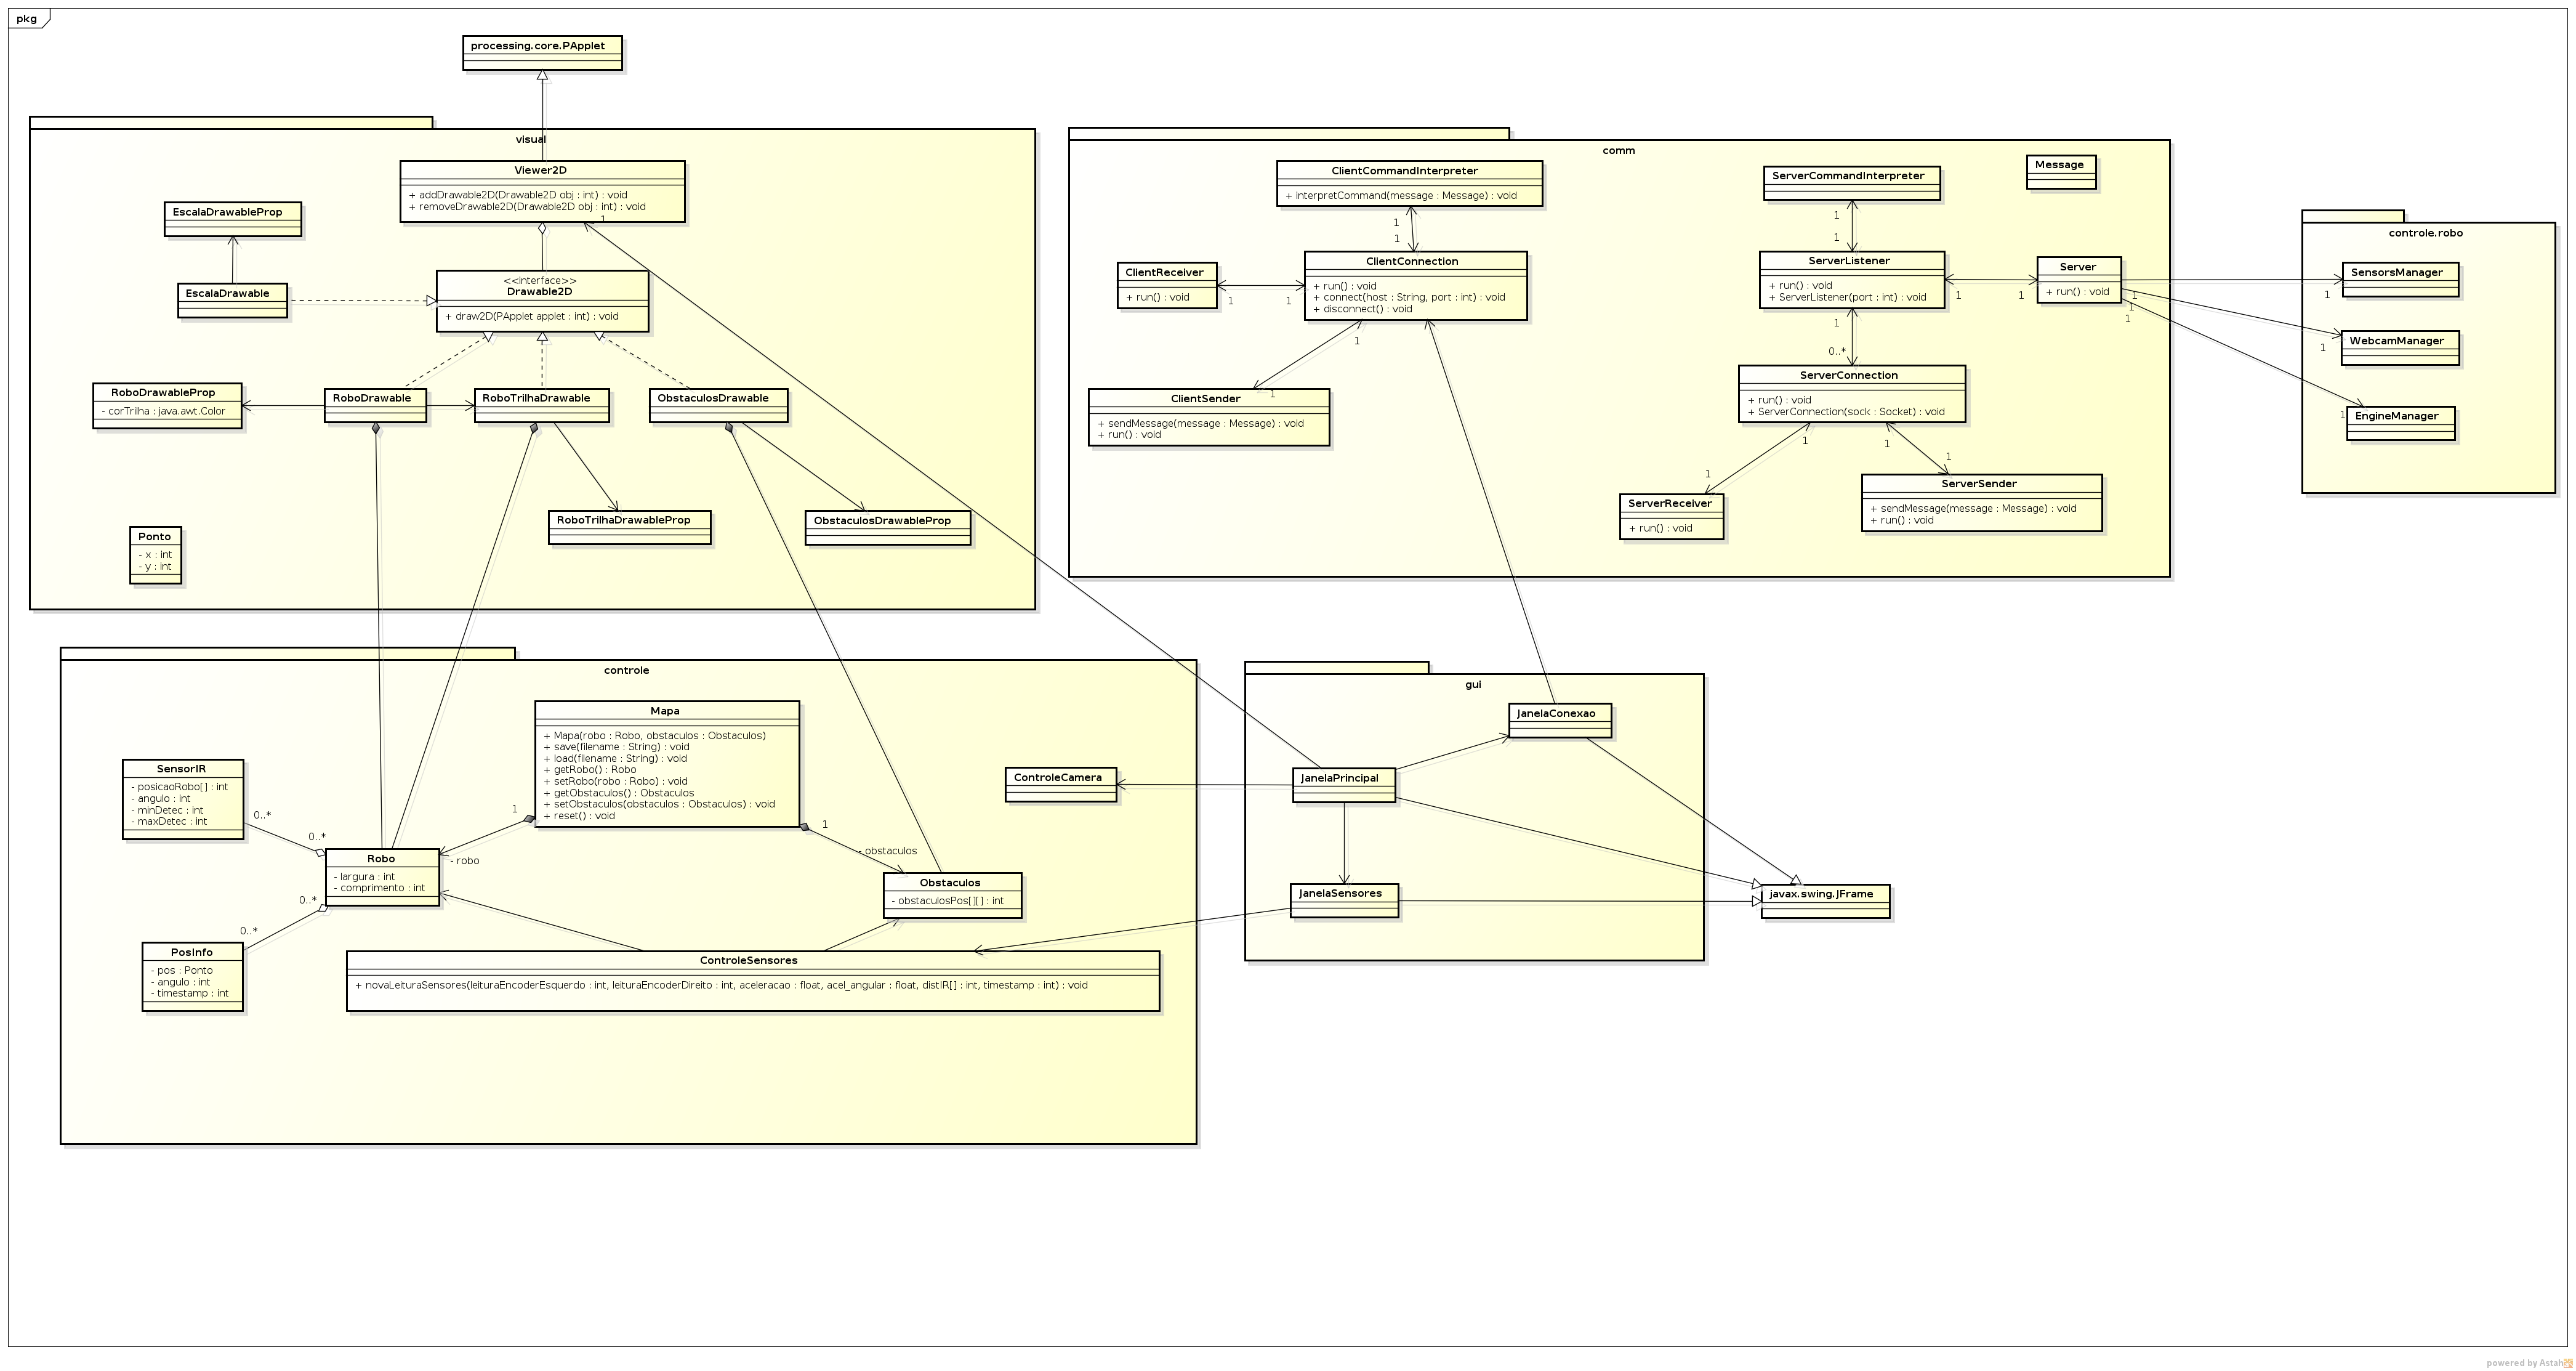
\includegraphics[width=\textwidth]{./figuras/diagrama_classes.png}
  \caption{Diagrama de classes}
  \label{fig:diagrama_classes}
\end{figure}
